\documentclass[10pt, fullpage, a4paper, titlepage]{article}
\usepackage{graphicx, latexsym}
\usepackage{subfigure}
\usepackage{setspace}
\usepackage{amssymb, amsmath, amsthm}
\usepackage{bm}
\usepackage{epstopdf}
\usepackage{rotating} %used for \sidewaystable
\usepackage{apacite}
\usepackage{booktabs} %used for \toprule
\usepackage{multirow} %used for \multirow and \multicolumn
\usepackage[]{hyperref}
\hypersetup{
    pdftitle={title of the pdf},
    pdfauthor={your name},
    pdfsubject={cool stuff},
    pdfkeywords={koala, chuck norris},
    bookmarksnumbered=true,     
    bookmarksopen=true,         
    bookmarksopenlevel=1,       
    colorlinks=true,      
    colorlinks=true,
    citecolor=blue,
    linkcolor=blue,
    urlcolor=blue,           
    pdfstartview=Fit,           
    pdfpagemode=UseOutlines,      
    pdfpagelayout=TwoPageRight
}

%\singlespacing
%\onehalfspacing
\doublespacing



\title{Examples}
\author{Gerko Vink}

\begin{document}
\maketitle
\newpage

When adding figures to \LaTeX, it is advisable to assign a \begin{verbatim}\label{figurelabelhere}\end{verbatim} When labels are set, referring to figures or even subfigures is child's play. For example, with \begin{verbatim}\ref{figurelabel}\end{verbatim}we can refer to Figure \ref{Fig1}, Figure \ref{Fig2}, Figure \ref{Fig3}, Figure \ref{Fig4}, Figure \ref{Fig5} or even Figure \ref{boxplot:a}, \ref{boxplot:b}, \ref{boxplot:c} or \ref{boxplot:d} 

\section{Figures in \LaTeX}
Please find below some examples of Figure placement and sizing with \LaTeX. 

%%%%%%%%%
% Figure 1        %
%%%%%%%%%
\begin{figure}[h]
  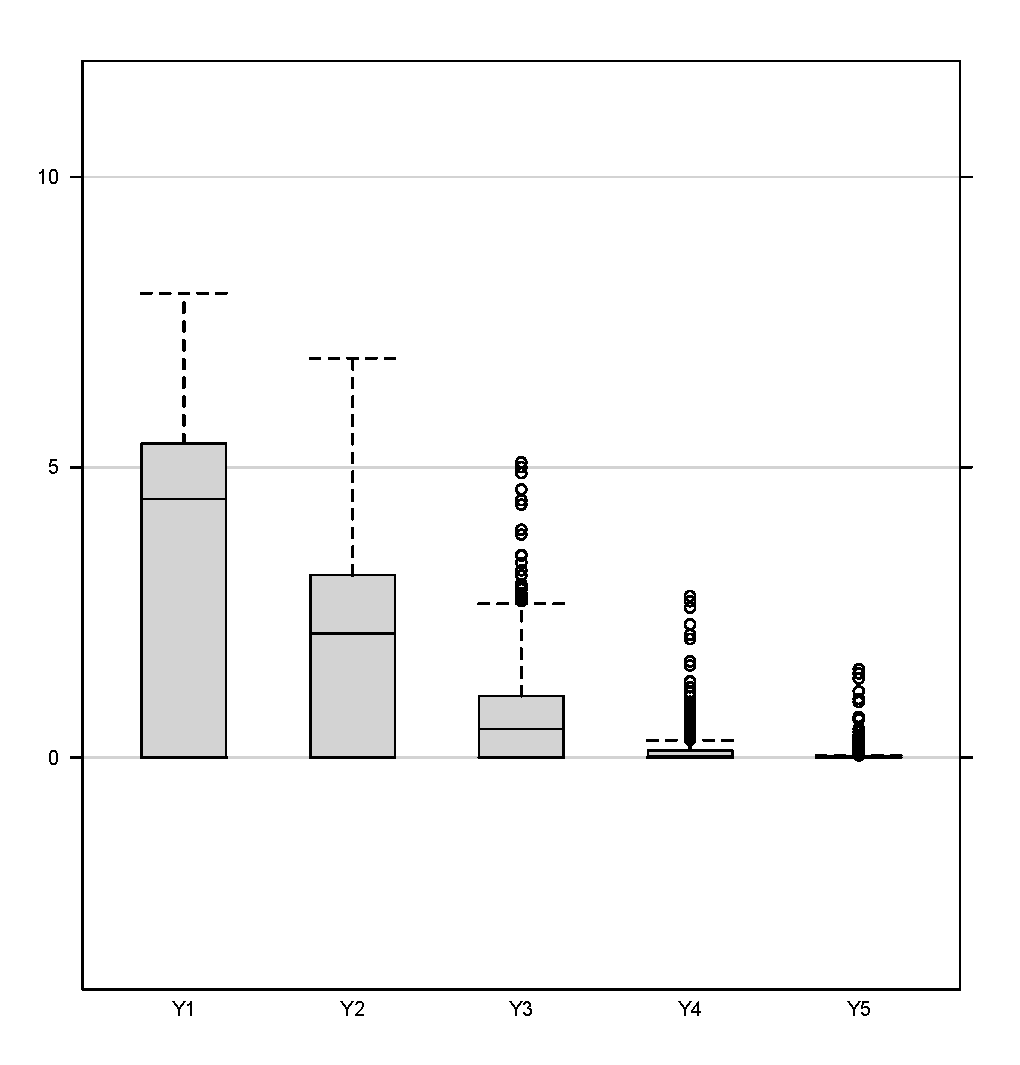
\includegraphics{Plots/Boxplot_pop_mr.pdf} %no [scale = �..] parameter
  \caption{Just a single figure. Too large.  }
  \label{Fig1}
\end{figure}
 
%%%%%%%%%
% Figure 2        %
%%%%%%%%%
\begin{figure}[h]
        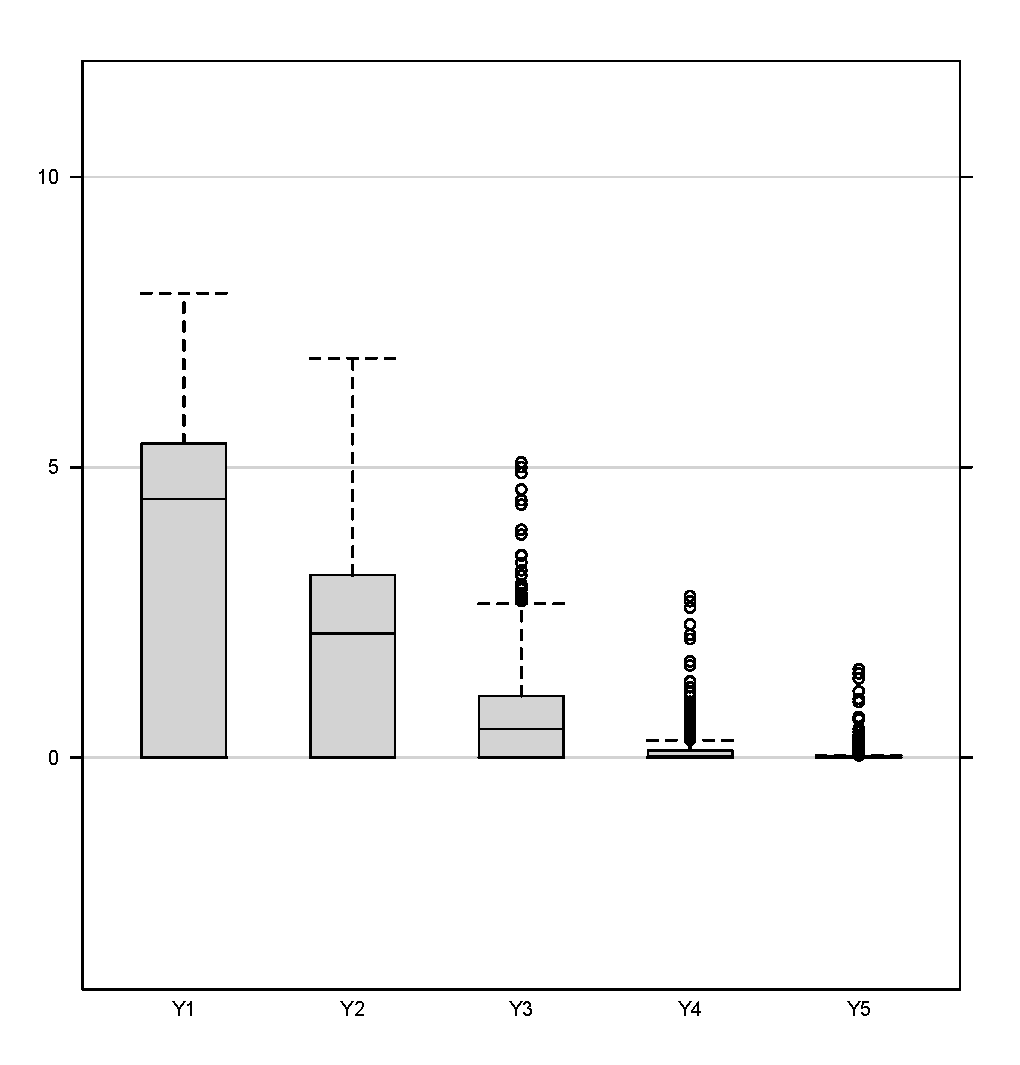
\includegraphics[scale = .5]{Plots/Boxplot_pop_mr.pdf} %notice the [scale = .5] scale parameter
  \caption{Just a single figure. Smaller (In fact, it is half its original size).  }
  \label{Fig2}
\end{figure}

%%%%%%%%%
% Figure 3        %
%%%%%%%%%

\begin{figure}[h]
        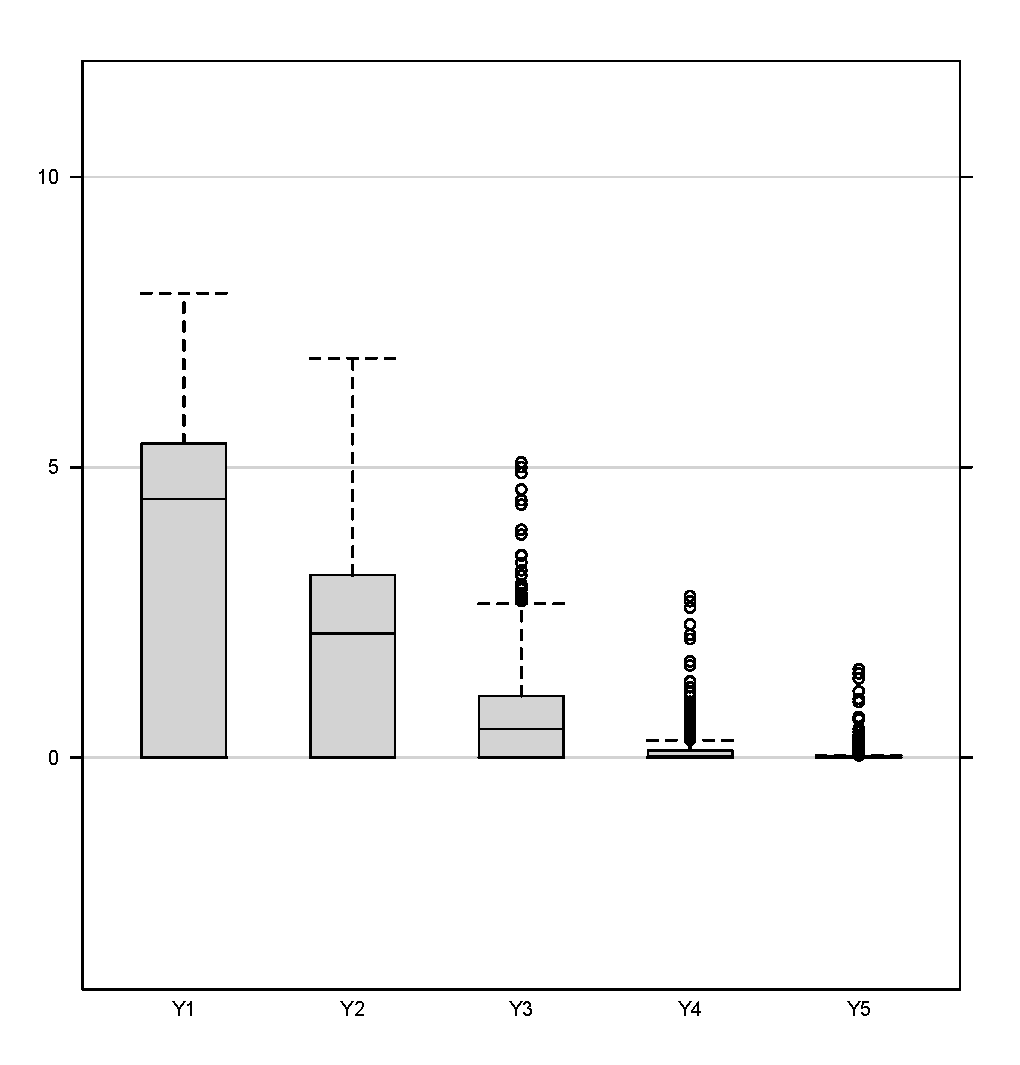
\includegraphics[scale = .75]{Plots/Boxplot_pop_mr.pdf} %notice the [scale = .75] scale parameter
  \caption{The same figure, now at $\frac{3}{4}$ its original size  }
  \label{Fig3}
\end{figure}

%%%%%%%%%
% Figure 4        %
%%%%%%%%%
\begin{figure}[h]
  \resizebox{\textwidth}{!}{ %notice the \resizebox{} command
        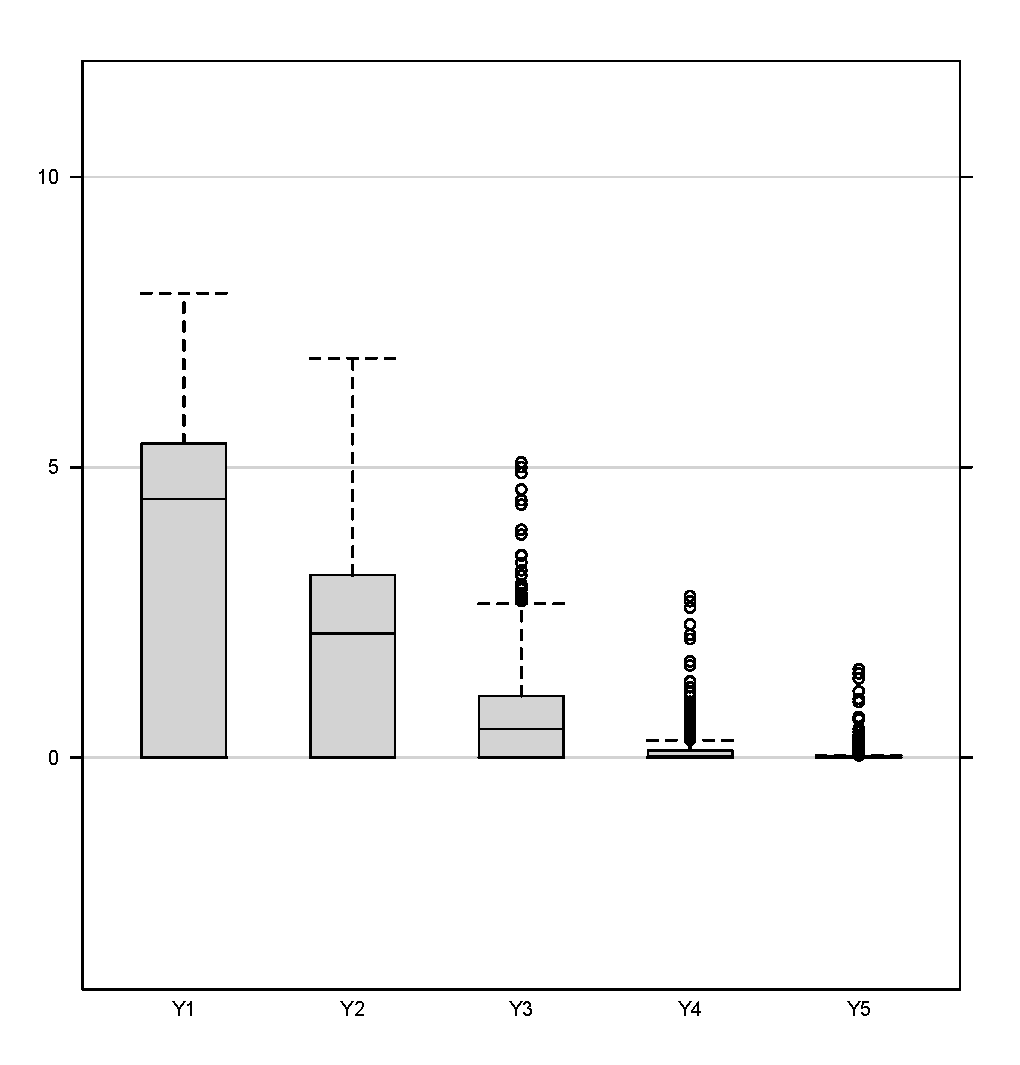
\includegraphics{Plots/Boxplot_pop_mr.pdf}
  }      
  \caption{The same figure again, but now at textwidth. This is much easier. It just borrows the width parameters from your document style's canvas.}
    \label{Fig4}
\end{figure}

%%%%%%%%%
% Figure 5       %
%%%%%%%%%
	\begin{figure}[h]
   	   \begin{center}
		\resizebox{\textwidth}{!}{
        			\subfigure[Original data]{
           			\label{boxplot:a}
  	  			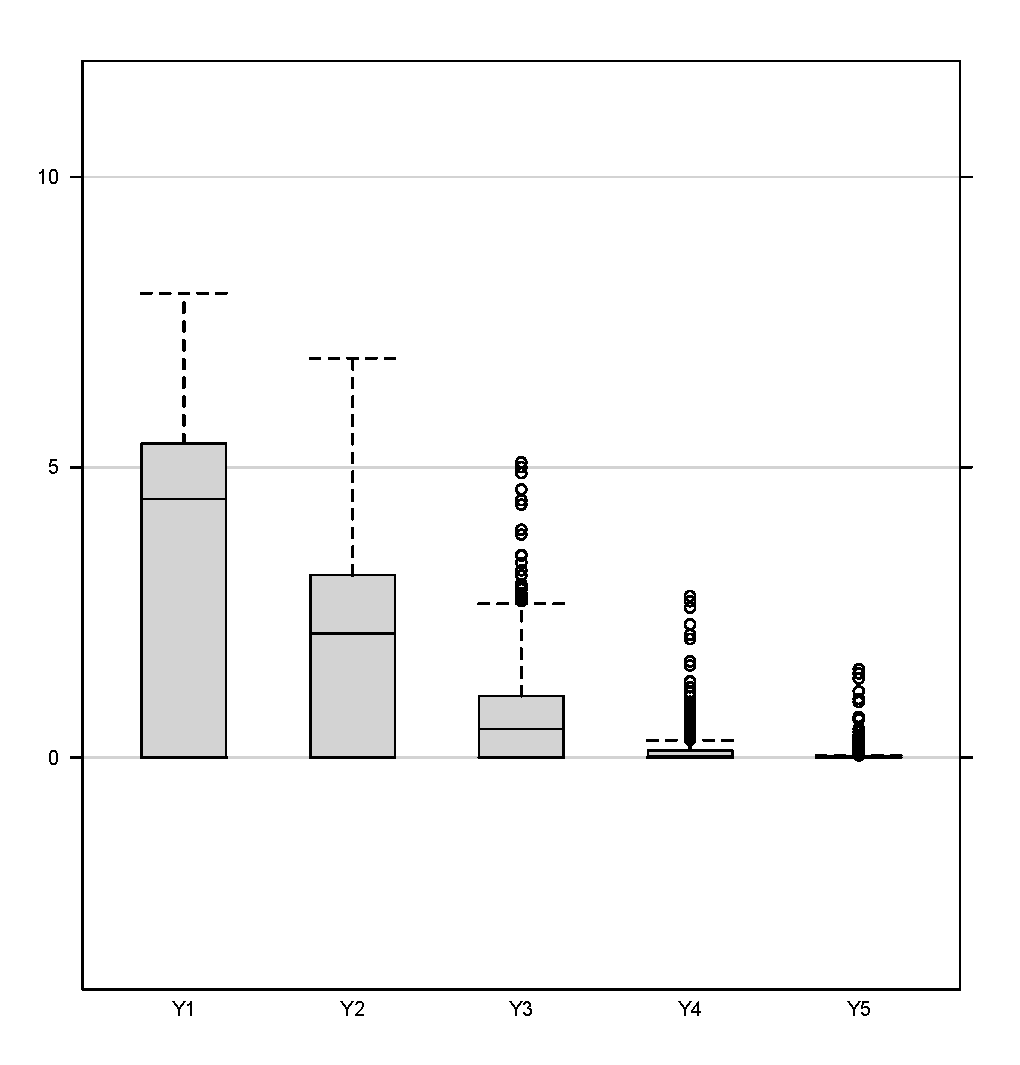
\includegraphics[scale=.5]{Plots/Boxplot_pop_mr.pdf}
        	                 }
        			\subfigure[PMM imputation]{
         		        \label{boxplot:b}
    				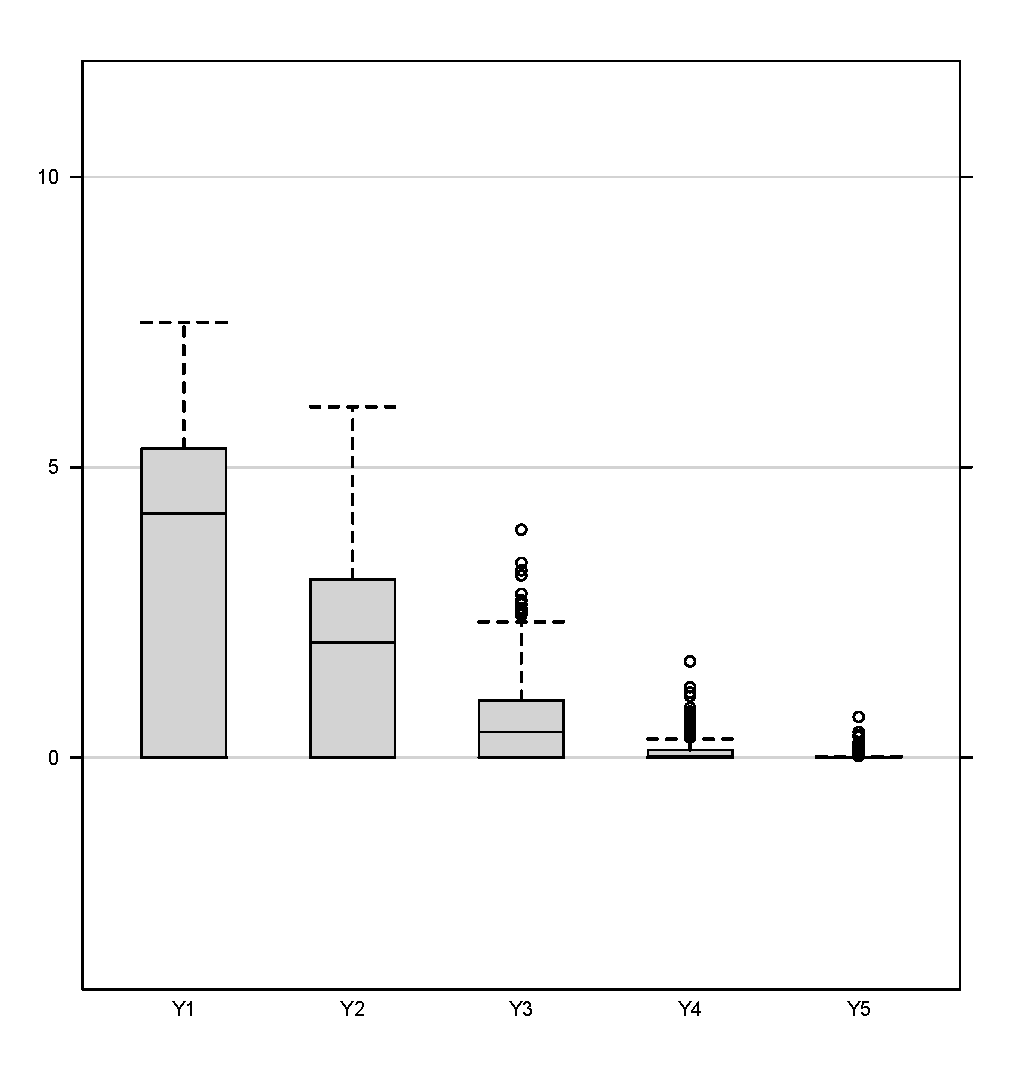
\includegraphics[scale=.5]{Plots/Boxplot_pmm_mr.pdf}
        		        }
		}\\ 	%  ------- End of the first row - hence the \\ ----------------------%
		\resizebox{\textwidth}{!}{
       			 \subfigure[BGLoM imputation]{
          		        \label{boxplot:c}
   	 			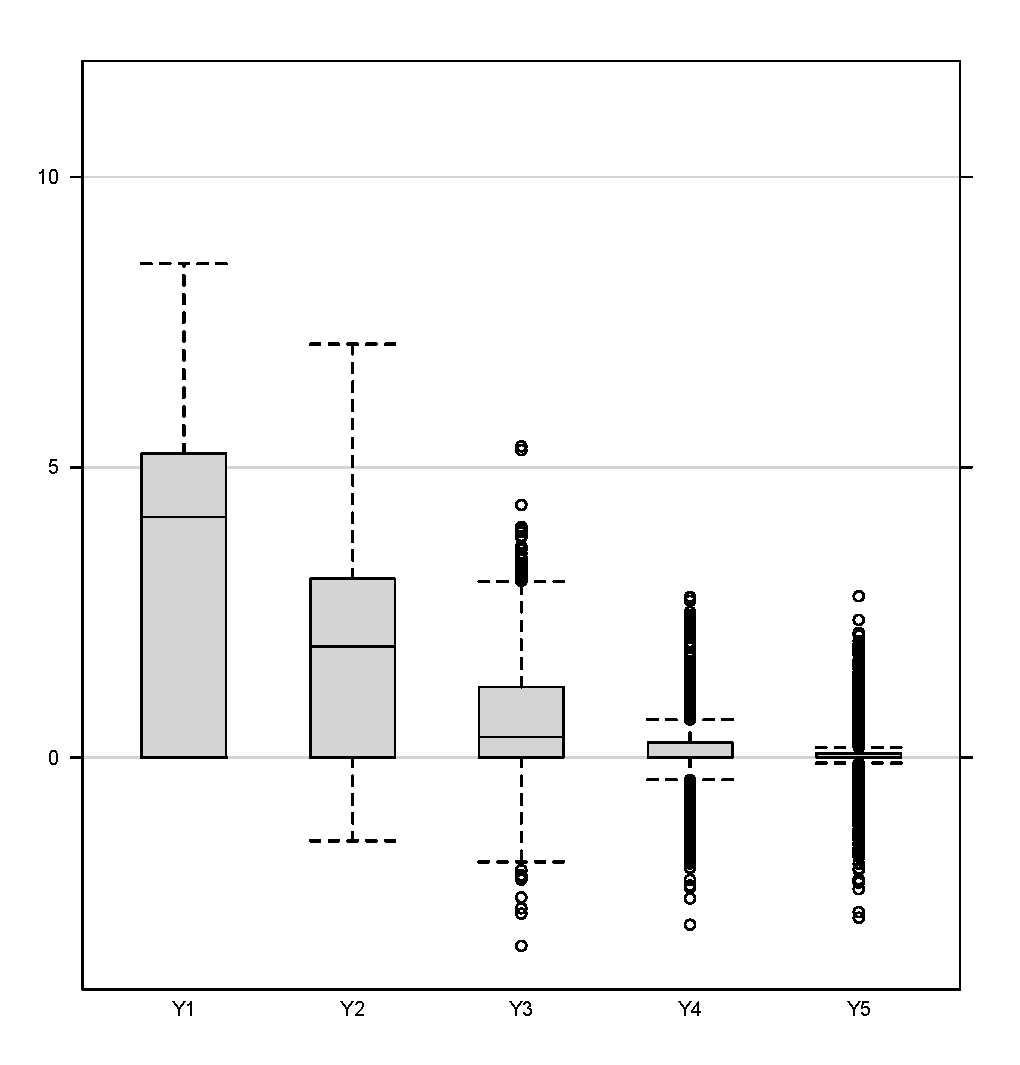
\includegraphics[scale=.5]{Plots/Boxplot_bglom_mr.pdf}
        			 }
       			 \subfigure[2-Step imputation]{
         		        \label{boxplot:d}
    				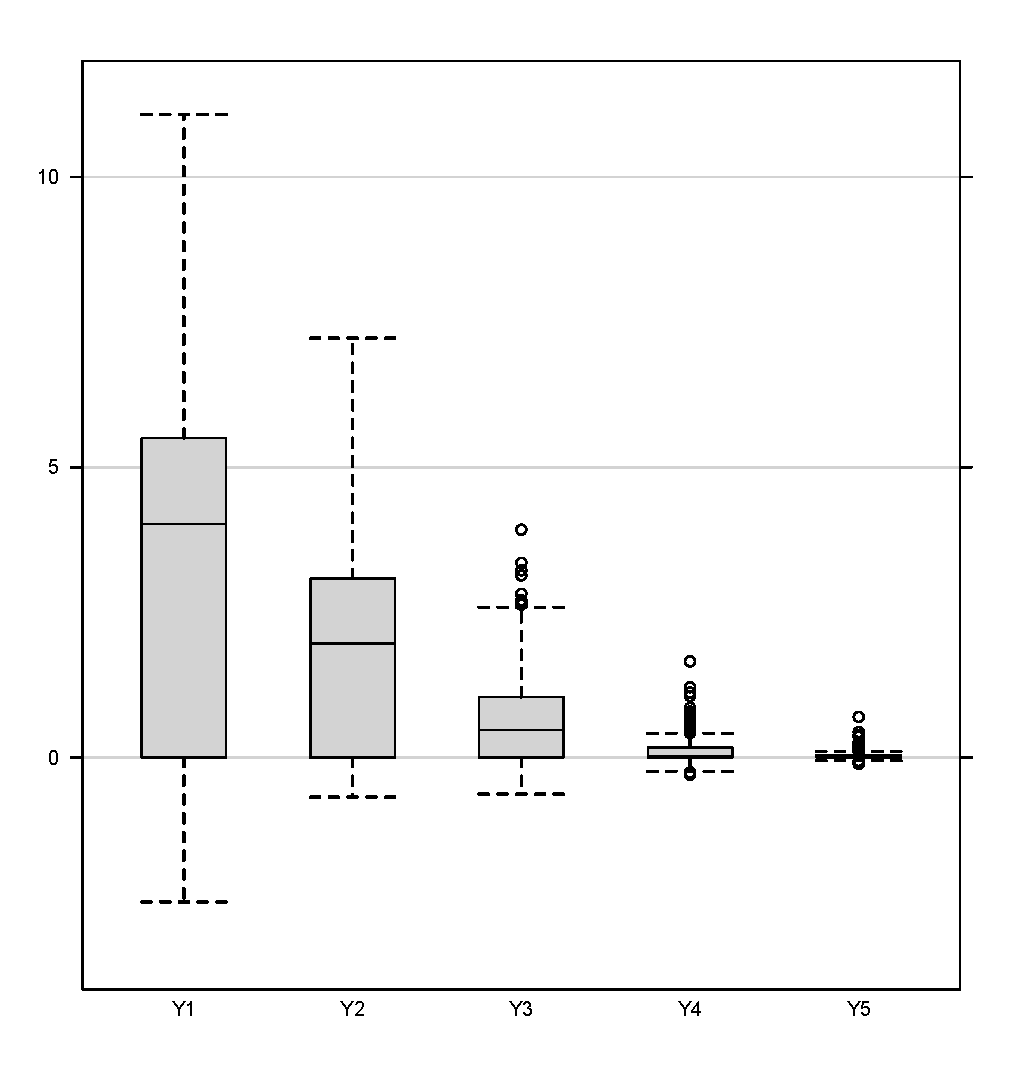
\includegraphics[scale=.5]{Plots/Boxplot_2step_mr.pdf}
			 }
		}
    	    \end{center}
    	\caption{Four different boxplots, each subset by (a) - (d). This subsetting - if properly labelled - can also be referred to by standard {\LaTeX}  referencing modes. }
     	  \label{Fig5}
	\end{figure}
	
\end{document}


